\chapter{Analýza kódu jazyka Java}

	\section{O jazyce Java}
		Java \cite{javaEnviroment} je objektově orientovaný programovací jazyk, který byl vytvořen více než před 20 lety. Java byla inspirována řadou jazyků, jako je např. Eiffel, SmallTalk a Objective C. Snahou bylo vytvořit objektově orientovaný jazyk, který bude jednoduchý na pochopení, aniž by bylo třeba dlouhého tréninku. Jedním ze značných usnadnění, např. oproti jazyku C/C++, je Garbage Collector. Ten umožňuje automatické uvolňování paměti, což předchází častým chybám spojených s jejím manuálním uvolňováním.	Cílem také bylo, aby byla Java robustní a zabezpečená a jednalo se tak o spolehlivý jazyk. Java byla vytvářena za účelem architektonické a platformní nezávislosti a bylo ji tak možné použít takřka všude. Této přenositelnosti bylo zajištěno především tím, že se jedná o interpretovaný jazyk (viž níže). Při vývoji bylo také samozřejmě cíleno na zajištění co největší výkonnosti s čímž souvisí i~umožnění tvorby vícevláknových aplikací.\\
		
		Java má řadu výhod ale také nevýhod a stejně jako u každé jiné technologie, je třeba zvážit, zda se jedná o vhodnou volbu pro náš projekt. Jazyk Java je dlouhodobě jedním z nejpoužívanějších programovacích jazyků a stále se vyvíjí \cite{javaTrend}.\\
		
		Tato kapitola bude čtenáře informovat o základních vlastnostech jazyka Java. Jejím hlavním cílem je představení gramatiky tohoto jazyka a úvod do problematiky tokenizace, která v důsledku umožní extrakci konstrukcí DbC. Dalším tématem budou také možnosti dekompilace bajtkódu a rozbor toho, jak se výsledek liší oproti zdrojovému kódu.
		
		
		\subsection{Kompilace jazyka Java}	
			Jazyk Java je tzv. interpretovaný jazyk, což znamená, že programovací kód není překládán přímo do strojového kódu daného zařízení, ale je přeložen do bajtkódu. Bajtkód je speciální vysoce-úrovňový kód, který je platformově nezávislý. V rámci kompilace Java to znamená, že zdrojové soubory \texttt{.java} jsou překompilovány do souborů \texttt{.class}. Výsledný Java program je pak distribuován ve formátu \texttt{.jar} nebo \texttt{.war}, což jsou prakticky archivy obsahující přeložené soubory. Na cílovém zařízení je pak program vykonáván pomocí \emph{Java Virtual Machine} (Virtuální stroj jazyka Java, dále JVM).
			
			\subsubsection{Java Virtual Machine (JVM)}			
				JVM je softwarová abstrakce pro obecnou hardwarovou platformu. Slouží k~tomu, aby bylo možné spustit program napsán v Java na různých zařízeních. Program je pak virtuálně spuštěn na JVM místo přímo na daném zařízení. Vzhledem k tomu, že se jedná o virtualizaci, je logické, že z hlediska výkonu a nároků na paměť není možné dosáhnout srovnatelných výsledků s programem, který je na danou platformu plně zoptimalizován. V tomto případě se jedná o daň za multiplatformnost jazyka Java.\\ 
			
			Když spustíme Java aplikace, nejprve se spustí JVM na daném zařízení. Ten načte hlavní třídu s metodou \texttt{main} spolu s jinými klíčovými částmi jako je např. \texttt{java.lang.Object}. K načtení těchto tříd se využívá tzv. \emph{Class Loader}. Poté, co jsou načteny klíčové části již JVM načítá třídy pouze na vyžádání, což se děje ve chvíli, kdy je daná třídy v programu potřeba. Tímto způsobem obsahuje JVM jen ten přeložený kód, který je v danou chvíli potřeba, což snižuje nároky na paměť, ale snižuje rychlost programu. 
		
	\section{Rozbor kódu}
		Abychom mohli zpracovávat zdrojový kód jazyka Java, je vhodné jej nejprve převést na snadněji zpracovatelnou formu než surový text. K tomu nám může pomoci lexikální a syntaktická analýza, pomocí nichž můžeme ve výsledku získat reprezentaci ve stromové podobě. Toho je běžně využíváno při tvorbě překladače a interpretu \cite{compilerTutorial}\cite{basicsOfCompilerDesign}\cite{fjp}.
			
		\subsection{Lexikální analýza}
			Aby bylo možné provést rozbor kódu, který je prezentován v textové podobě, je třeba nejprve provést lexikální analýzu. Ta spočívá v tom, že je proud znaků zpracováván a rozdělován do tzv. lexémů. Lexém je posloupnost znaků, která tvoří ucelenou část kódu (např. číslo, název proměnné atd.). Lze je rozdělit do různých kategorií: identifikátory, klíčová slova (rezervované identifikátory), čísla, jednoznakové omezovače atd.\\
			
			Zpracování začíná prvním dosud nezpracovaným znakem ze vstupu. Končí ve chvíli, kdy se nacházíme v koncovém stavu a již není možné přidat další znak. Tím je daná posloupnost znaků uzavřena a tvoří tak jeden lexém. Např. při zpracování kódu \texttt{var+4} začneme zpracovávat písmenem \texttt{v} a postupujeme dál přes \texttt{a} a \texttt{r}. Písmenem může začít pouze identifikátor nebo klíčové slovo. Ve chvíli, kdy dojdeme k \texttt{+}, víme, že je tento lexém kompletní, protože znak \texttt{+} nemůže být součástí identifikátoru resp. klíčového slova. Rozlišení, zda se jedná o identifikátor nebo klíčové slovo je řešeno pomocí tabulky klíčových slov.\\
			
			Toto zpracování se řídí definovanou gramatikou jazyka. Protože se jedná o gramatiku typu 3, je možné jí nahradit regulárními výrazy. Pokud by analyzátor narazil na neplatný symbol v dané posloupnosti, je vyhozena chyba. Lexikální analýza není schopna odhalit chybu, jako např. že není platná posloupnost \texttt{* *}, protože se jedná o dva platné lexémy. Ve chvíli, kdyby by se jednalo o text \texttt{**}, vznikne chyba, protože to není platný tvar z~hlediska regulárního výrazu. Seznam lexémů je dále předáván ke zpracování syntaktické analýze.
			
				\begin{figure}[!htb]
					\minipage{1\textwidth}	
						\centering
						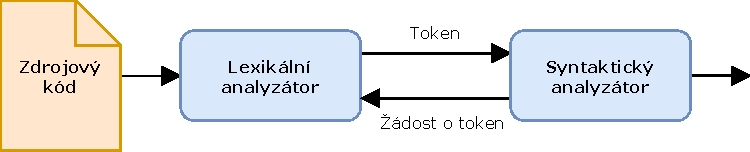
\includegraphics[width=1\textwidth]{img/lexicalAnalysis.pdf}
						\caption[lexicalAnalysis]{Princip lexikální analýzy}
						\label{lexicalAnalysis}
					\endminipage\hfill
				\end{figure}			
			
		\subsection{Syntaktická analýza}
			Ve chvíli, kdy je text převeden do lexémů pomocí lexikální analýzy, je možné provést syntaktickou analýzu, někdy nazývanou parsování. Lexikální analýza není schopna kontrolovat syntaxi kvůli limitacím regulárních výrazů. Syntaktická analýza však pracuje na úrovni bezkontextové gramatiky, která je té regulární nadřazená, proto to umožňuje. Na obrázku \ref{bkg} je možné vidět ukázku této gramatiky. Velká písmena (\texttt{S}, \texttt{Z}, \texttt{E}, ..) představují neterminální symboly, jejichž výčet je na levé straně obrázku. Za šipkou pak následuje, na co je možné dané neterminální symbol přepsat. To často mohou být další neterminální symboly a celý výraz se takto rozrůstá. Svislými čarami (\texttt{|}) jsou odděleny možnosti, na které se může symbol přepsat. Symbol \texttt{F} tedy může být rozepsán na \texttt{(E)} nebo na \texttt{V}.\\
			
			Ostatní řetězce (zde \texttt{if}, \texttt{then}, \texttt{\{}, ...) jsou potom terminální výrazy, které jsou konečné a nejde je dále rozepsat. Symbol malé \texttt{e} je speciální a představuje prázdný znak, který ukončuje danou posloupnost. Pomocí symbolů \texttt{+} a \texttt{*} je možné vyjádřit opakování daného výrazu. Tímto způsobem je tedy možné vyjádřit gramatiku programovacího jazyka. Pokud vstupní lexémy neodpovídají této gramatice, vzniká syntaktická chyba.
			
			\begin{figure}[!htb]
				\minipage{1\textwidth}	
					\centering
					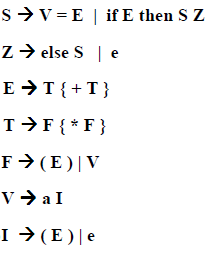
\includegraphics{img/gramatika.png}
					\caption[bkg]{Ukázka bezkontextové gramatiky}
					\label{bkg}
				\endminipage\hfill
			\end{figure}
			
			Jedním ze způsobů, jak zpracovávat tuto gramatiku je rekurzivní sestup. Každý z neterminálních symbolů je prezentován procedurou, která se vykoná, ve chvíli, kdy se jedná o daný symbol. Takto se postupně rekurzivně volají procedury dokud není zpracován celý vstup. V proceduře s terminálním souborem pak můžeme vykonat určitou akci, která koresponduje s~daným výrazem, např. přidat do seznamu další strojovou instrukci. Pro rozhodování je použita technika, kdy se nahlíží na další lexémy na vstupu a podle toho se určí o jaký výraz se jedná. Gramatika musí být vždy jednoznačná.
			
		\subsection{Nástroje}
			I přesto, že by bylo možné provádět zmíněné analýzy pomocí vlastního kódu, je také možné použít některý z dostupných nástrojů. Tyto nástroje umožňují parsování zdrojového kódu za použití samostatné aplikace nebo se může jednat o knihovnu, jejíž API můžeme použít přímo v našem kódu.
			
			\paragraph{JFLex}
				JFLex \cite{jflex} je lexikální analyzátor pro jazyk Java. Protože lexikální analýza sama o sobě nestačí k analýze kódu vhodné pro detekci kontraktů, je třeba tento nástroj použít s jiným, který umožní syntaktickou analýzu. Může se jednat např. o ANTLR, BYacc/J či CUP. 						
						
			\paragraph{ANTLR}			
				ANTLR \cite{antlr} je široce používaný nástroj, který umožňuje na základě zadané gramatiky vytvořit a procházet strom daného zdrojového kódu. ANTLR je primárně určen ke zpracování vlastní gramatiky např. při tvorbě vlastního překladače, nicméně je možné také použít gramatiku jazyka Java pro rozbor jejího zdrojového kódu.
			
			\paragraph{JavaParser}
				JavaParser \cite{javaparser} je jedním z dostupných nástrojů, který umožňuje analýzu, parsování ale i konstruování kódu jazyka Java. Funguje jako knihovna, kterou můžeme použít v našem kódu. Jedná se o vyspělou technologii, která je použita v řadě projektů. 
				
			\paragraph{Roaster}
				Roaster \cite{roaster} je nástroj podobný JavaParser. Také umožňuje nejen parsování, ale i editaci zdrojových kódů jazyka Java. Mimo dostupného API umožňuje také práci s konzolí  pro jednoduché použití.
	

	\section{Gramatika jazyka Java}
		Vzhledem k tomu, že Java je plnohodnotný programovací jazyk s řadou funkcí, je jeho specifikace gramatiky \cite{javaGrammar} velice rozsáhlá. V této části budou pouze vyzdviženy některé informace, které mohou být důležité pro problematiku extrakce kontraktů. Tyto informace budou vycházet ze specifikace Java verze 1.8, nicméně by měly být shodné i s ostatními verzemi současné doby.\\
		
		Java je definována dvěma bezkontextovými gramatikami. Jedna z nich je lexikální a ta specifikuje, jak vypadají jednotlivé lexémy. Určuje, co může obsahovat identifikátor, jaká jsou klíčová slova, omezovače atd. Této části zde nebude věnována velká pozornost. Naopak druhou gramatikou, která je z hlediska extrakce kontraktů důležitější, je syntaktická gramatika.
		 
		\subsection{Syntaxe}
			Syntaxe určuje, jaké posloupnosti lexémů jsou povolené pro správně fungující program. Protože se stále jedná o gramatiku, bude se při popisu vycházet z~toho, že se daný úsek vždy skládá z neterminálů, které se přepisují na terminály a neterminály. Terminály (např. \texttt{\textcolor{pblue}{class}}) jsou konečné prvky, které není dále možné rozvíjet, zatímco neterminály (např. \texttt{ClassModifier}) zastupují jiné neterminály a terminály. Neterminál uzavřený v hranatých závorkách (\texttt{[]}) se může vyskytnou nejvýše jedenkrát. Složené závorky (\texttt{\{\}}) pak určují, že se daný neterminál může vyskytnout nejvýše n-krát. Pravá strana rozdělená do více řádek je pouze příliš dlouhá než aby se na daný řádek vešla. Nejedná se alternativní možnost přepisu. Ty jsou vždy rozděleny symbolem svislé čáry (\texttt{|}).
			
			\subsubsection{Kompilační jednotka}	
				Výchozím bodem je tzv. \emph{compilation unit}, nebo-li kompilační jednotka. Z~hlediska gramatiky se jedná o nejobecnější neterminál, jinak řečeno počáteční symbol, ze kterého vycházejí všechny ostatní neterminály. V praxi se jedná o zdrojový soubor jazyka Java.\\\\
				\- \- \- \- \- \- \texttt{CompilationUnit $\rightarrow$}\\
				\- \- \- \- \- \- \- \- \- \- \- \- \texttt{[PackageDeclaration] \{ImportDeclaration\} \{TypeDeclaration\}}\\
				
				Zde je vidět, že se kompilační jednotka skládá z deklarace balíčku, deklarace importů a deklarace typu. Deklarace balíčku je jedna volitelná položka, kterou lze použít ke specifikaci toho, v jakém balíčku se tento soubor nachází. Neterminál \texttt{ImportDeclaration} představuje importy, kterých může být libovolné množství. Symbol \texttt{TypeDeclaration} pak představuje deklaraci rozhraní nebo deklaraci třídy. Samotná deklarace třídy se pak ještě dělí na deklaraci výčtového typu a deklaraci běžné třídy.
			
			\subsubsection{Deklarace třídy}
				Třídy představují základní stavební jednotku objektového jazyka Java. Z~hlediska syntaxe zde bude popsána deklarace běžné třídy, nicméně deklarace rozhraní a výčtového typu jsou v mnoha ohledech podobné.\\\\
				\- \- \- \- \- \- \texttt{NormalClassDeclaration $\rightarrow$}\\
				\- \- \- \- \- \- \- \- \- \- \- \- \texttt{\{ClassModifier\} \textcolor{pblue}{class} Identifier [TypeParameters]}\\  	 
				\- \- \- \- \- \- \- \- \- \- \- \- \texttt{[Superclass] [Superinterfaces] ClassBody}\\
	
				Neterminál \texttt{ClassModifier} zde představuje modifikátor třídy. Mohou zde být definovány anotace (viz níže) a také určení, zda je daná třída veřejná či privátní, zda je abstraktní, statická atd. Symbol \texttt{Identifier} reprezentuje identifikátor nebo-li pojmenování dané třídy. To musí být unikátní jinak nastává kompilační chyba. \texttt{TypeParameters} představuje typové určení ve špičatých závorkách (např. \texttt{List<String>}). V případě \texttt{Superclass} se pak jedná o dědičnost (tedy \texttt{extendes NAZEV}) a \texttt{Superinterfaces} zastupuje implementace rozhraní (tedy \texttt{implements NAZEV}). Položka \texttt{ClassBody} představuje celé tělo třídy, jsou tu tedy atributy, konstruktory, metody atd.	 
		 
			\subsubsection{Deklarace metody}
				Metoda se z hlediska gramatiky skládá ze tří složek. Nejprve jsou zde modifikátory metody \texttt{MethodModifier}. Jedná se o stejné položky jako v případě třídy, tedy anotace a definice \texttt{private/protected/public}, \texttt{static}, \texttt{final} atd. Neterminál \texttt{MethodHeader} představuje hlavičku metody, ta je podrobněji popsána dále. Poslední částí je \texttt{MethodBody}, tedy tělo metody. To se skládá z bloku kódu, který je z hlediska syntaxe velice komplexní. Jsou zde podmínky, cykly, volání metod, definice proměnných atd.\\\\
				\- \- \- \- \- \- \texttt{MethodDeclaration $\rightarrow$}\\
				\- \- \- \- \- \- \- \- \- \- \- \- \texttt{\{MethodModifier\} MethodHeader MethodBody}\\\\
 				\- \- \- \- \- \- \texttt{MethodHeader $\rightarrow$}\\
				\- \- \- \- \- \- \- \- \- \- \- \- \texttt{Result MethodDeclarator [Throws]}\\\\
				\- \- \- \- \- \- \texttt{MethodDeclarator $\rightarrow$}\\
				\- \- \- \- \- \- \- \- \- \- \- \- \texttt{Identifier ( [FormalParameterList] ) [Dims]}\\

				Hlavička metody tvoří hlavní část její signatury. Symbol \texttt{Result} představuje návratový typ metody. \texttt{Throws} umožňuje propagaci výjimek pomocí klíčového slova \texttt{throws}. Neterminál \texttt{MethodDeclarator} se pak dále člení. \texttt{Identifier} opět představuje identifikátor, tedy jméno dané metody. V závorce jsou pak uvedeny jednotlivé parametry. Ty se typicky skládají z definice typu a identifikátoru. Volitelné jsou pak opět různé modifikátory včetně anotací.	
 		
			\subsubsection{Deklarace anotace} 
				Běžné anotace jsou definovány pouze symbolem \texttt{@} následovaným názvem anotace. Poté je možné volitelně do závorek uvést další parametry. Symbol \texttt{TypeName} reprezentuje název, ten musí představovat validní anotaci, jinak nastane chyba. Za názvem s v závorce mohou nacházet další parametry. Neterminál \texttt{ElementValue} představuje jednu položku hodnoty anotace. Může se jednat o libovolný objekt, pole, další anotaci, ternární výraz atd. \texttt{ElementValuePairList} pak představuje seznam přiřazení typu: \texttt{identifikátor = hodnota}.\\\\\\
				\- \- \- \- \- \- \texttt{Annotation $\rightarrow$}\\
				\- \- \- \- \- \- \- \- \- \- \- \- \texttt{\textcolor{pblue}{@} TypeName |}\\
				\- \- \- \- \- \- \- \- \- \- \- \- \texttt{\textcolor{pblue}{@} TypeName ( ElementValue ) |}\\
				\- \- \- \- \- \- \- \- \- \- \- \- \texttt{\textcolor{pblue}{@} TypeName ( [ElementValuePairList] )}\\		
	
	\section{Retenční politika anotací}		
				\emph{Retention Policy} \cite{retentionPolicy}, nebo-li retenční politika, určuje, v jaké chvíli mají být anotace odebrány z programu. V Java existují tři typy retenčních politik, jsou uchovány ve výčtovém typu \texttt{java.lang.annotation.RetentionPolicy}: 
					
					\begin{itemize}
						\item \texttt{SOURCE}
						\item \texttt{CLASS}
						\item \texttt{RUNTIME}
					\end{itemize}
					
				Anotace s retenční politikou \texttt{SOURCE} bude uchována pouze ve zdrojovém kódu a během kompilace bude zahozena. Politika \texttt{CLASS} říká, že anotace zůstane zachována během kompilace, ale je zahozena při běhu programu. Retenční politika \texttt{RUNTIME} pak zajišťuje, že bude anotace dostupná i při běhu programu. Výchozí hodnotou je \texttt{CLASS}. To je možné změnit při definici dané anotace využitím jiné anotace \texttt{@Retention}. To je možné vidět na příkladu níže.\\\\
				\- \- \- \- \- \- \texttt{@Retention(RetentionPolicy.RUNTIME)}\\
				\- \- \- \- \- \- \texttt{public @interface MySampleAnnotation \{}\\
				\- \- \- \- \- \- \- \- \- \texttt{...}\\
				\- \- \- \- \- \- \texttt{\}}\\

				Pokud nemají anotace retenční politiku \texttt{SOURCE}, jsou také zaneseny do bajtkódu. Jedná se tedy o podmínkou proto, abychom mohli extrahovat kontrakty definované anotacemi z přeložených souborů. Např. anotace reprezentací JSR305 mají retenční politiku \texttt{RUNTIME} a jsou tedy uchovány v~bajtkódu.
	
	\section{Rozbor přeložených souborů}
		Při analýze kontraktů v jiných projektech není vždy možné získat zdrojové soubory. Z toho důvodu je užitečné umět analyzovat nejen soubory \texttt{.java}, ale také přeložené soubory \texttt{.class}.
	
		\subsection{Dekompilace}
			Aby bylo možné soubory analyzovat, musíme je nejprve dekompilovat. Dekompilace je vlastně opačný proces kompilace a jejím cílem je tedy získat původní zdrojový kód z cílové podoby. Tou bývají obvykle strojové instrukce, v případě Java se jedná o bajtkód. Výhodou bajtkódu je, že obsahuje vysoké množství různých podrobností, které umožňují téměř bezztrátovou rekonstrukci zdrojového kódu. Jednoduchý princip je vidět na obrázku \ref{decompilation}.
			
			\begin{figure}[!htb]
				\minipage{1\textwidth}	
					\centering
					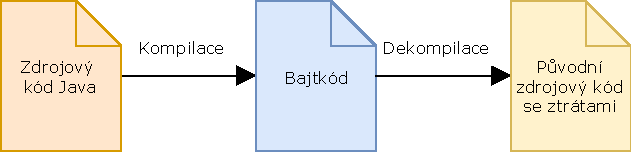
\includegraphics{img/decompilation.pdf}
					\caption[decompilation]{Dekompilace}
					\label{decompilation}
				\endminipage\hfill
			\end{figure}
			
			\subsubsection{Nástroje}
				Nástrojů pro dekompilaci souborů v jazyce Java je celá řada. Některé je nutné pouštět samostatně, ty pak mohou být vytvořeny i v jiných programovacích jazycích. Vývojová prostředí jako např. Eclipse či IDEA IntelliJ umožňují instalaci balíčků, které podporují dekompilaci souborů. Některé z~nástrojů je také možné použít přímo v kódu formou knihovny. Následuje seznam některých dostupných nástrojů, které jsou stále aktualizovány a umožňují dekompilaci moderních prvků jazyka Java \cite{top8decompilers}\cite{decompilersOnline}\cite{quickDecompilers}.	
				
				\paragraph{JD Project}
					JD Project (Java Decompiler) \cite{jd} je jedním z nejčastěji referovaných nástrojů v rámci Java dekompilace. JD disponuje samostatnou aplikací s grafickým uživatelským rozhraním, pomocí kterého je možné soubory dekompilovat a ihned vidět výsledek. JD také poskytuje doplněk do Eclipse a IDEA IntelliJ. Nejedná se o open-source nástroj, ale je dostupný zdroj pro GUI aplikaci. Nástroj bohužel nedisponuje API, aby bylo možné jej použít přímo v kódu.
					
				\paragraph{Procyon}
					Procyon \cite{procyon} je open-source nástroj, který také umožňuje dekompilaci. Nemá samostatné GUI jako JD, nicméně je možné reprezentaci zobrazit použitím externích nástrojů. Disponuje také API, které je možné použít přímo v kódu. Stačí zavolat metodu \texttt{decompile()}, kam vstupuje jméno souboru, který chceme dekompilovat a také kam má být směrován výstup. Výsledkem je pak zdrojový kód. Nejedná se samozřejmě přesnou kopii, ale jsou zde jisté limitace (viz níže).
					
				\paragraph{CFR}
					CFR \cite{cfr} je dalším z nástrojů, který umožňuje dekompilaci i konstrukcí Java 1.9. Nástroj je možné použít pouze v rámci příkazové řádky, kdy je na výstup směrován dekompilovaný kód. Součástí tedy není API, které by umožnilo použití v kódu.\\
					
				Nástrojů pro dekompilaci jazyka Java je velké množství a jejich výběr není snadný zejména poroto, že se neustále vyvíjejí na základě nových verzí Java. Při výběru je samozřejmě také důležité, jakým způsobem je daný nástroj možné používat, jaké konstrukce dokáže dekompilovat a roli může hrát také rychlost.
				
			\subsubsection{Rozdíly oproti původním souborům}
				Jak již bylo zmíněno, velice závisí na použitém nástroji pro dekompilaci. Jestliže daný nástroj nepodporuje určité konstrukce, pak je logické že jejich dekompilace nebude možná a není tak možné získat původní zdrojový soubor. Pokud nástroj umožňuje dekompilaci všech použitých konstrukcí, výsledný kód stále nebude zcela shodný. Přeložený kód obsahuje plné cesty k objektům, doplňuje neuvedená přetypování atd. Tyto informace často ve zdrojových kódech nebývají uvedené, protože jsou redundantní, ale při rekonstrukci přeloženého souboru není možné určit, kde tyto informace byly a~kde ne. Přirozeně také není možné získat data, která se do bajtkódu nezanášejí, jako jsou např. komentáře.